\documentclass[10pt, journal, letterpaper]{IEEEtran}
%\IEEEoverridecommandlockouts
% The preceding line is only needed to identify funding in the first footnote. If that is unneeded, please comment it out.
\usepackage{cite}
\usepackage{amsmath,amssymb,amsfonts}
\usepackage{algorithmic}
\usepackage{graphicx}
\usepackage{textcomp}
\usepackage{xcolor}
\usepackage{subfigure}
\usepackage{amsmath}
\usepackage{algorithm}
\usepackage{algorithmic}
\usepackage{caption}
\usepackage{booktabs}
\usepackage[colorlinks,linkcolor=black,anchorcolor=black,citecolor=black]{hyperref}
\captionsetup[figure]{labelformat=simple}
\renewcommand{\algorithmicrequire}{ \textbf{Input:}} %Use Input in the format of Algorithm
\renewcommand{\algorithmicensure}{ \textbf{Output:}} %UseOutput in the format of Algorithm


\usepackage{mathtools}
\DeclarePairedDelimiter{\ceil}{\lceil}{\rceil}


\begin{document}

\title{Solution to PS-004 in ITUChallenge 2021\\
% \thanks{\\
% }
}


\author{\IEEEauthorblockN{Hao Chen$^{\dag}$, Xiaoying Ye$^{\dag}$, Lizhao You$^{\dag}$, and Yulin Shao$^{\S}$\\}
\IEEEauthorblockA{$^{\dag}$School of Informatics, Xiamen University\\
	$^{\S}$Department of Electrical and Electronic Engineering, Imperial College London\\
Email: \{chenhao24,~yexiaoying0714\}@stu.xmu.edu.cn, lizhaoyou@xmu.edu.cn, linton.ylshaw@gmail.com}}


\maketitle

\section{WirelessAI}

We follow the Federated Learning (FL) framework to address the complex spatial reuse (SR) problem in multiple 11ax WLAN cells. Individual agents first train their local neural network (NN) models (with the same network structure) using their local datasets, and then exchange and average model weights through a centralized parameter server. 

{\bf NN Models}: Typical neural network (NN) models use simple data structure such as vectors to encode inputs and outputs. However, in wireless networks characterized by graphs $G=(V,~E)$, where $V$ is the set of nodes, and $E$ is the set of wireless links, the number of nodes and the number of links can vary depending on the networking scenarios. It is difficult to fix the vector dimension to fit all networking scenarios. Even if we can fix the dimension and pad zeros to the unused dimension fields, it is meaningless to use these fields.

To overcome the graph representation problem, we treat the whole network as an image. More specially, we first fix a maximum range, and treat the whole network as a 1$\times$100$\times$100 gray-scale image with default value 0. Then we map nodes to values by their roles (i.e., AP role with value 1, the target AP with OBSS/PDD value, other APs with value 1, and STAs with value 2), and place the values to their corresponding locations. In this way, we can represent any networks with arbitrary APs and STAs. Note that the topology information is encoded into the image.

Then, we adopt two NNs to predict the performance: one part is Convolutional Neural Network (CNN), and the other part is Fully Connected Neural Network (FCNN). We first use CNN to capture the interactions between STAs and APs to predict the RSSI, Signal to Interference plus Noise Ratio (SINR) of the BSS of interest and interference to the AP of interest. The input of the CNN is the above processed gray-scale image, and the used OBSS/PD value, and the output of the CNN is the RSSI, SINR, and the caused interference. Then, we use the output of CNN as the input of FCNN to predict the downlink throughput of the AP of interest. 

The key rationale of using such architecture is to reduce computation complexity. RSSI, SINR, and the caused interference are the key factors that impact the final performance. Compared with using a whole FCNN to predict the performance, if we can first use CNN to model the relationship among \{topology, OBSS/PD value\} and \{RSSI, SINR, and the caused interference\}, and then use a small dimension of FCNN to predict the performance, the computation complexity is reduced.


{\bf Federated Learning Algorithm}: We treat each context as a local client, and let each local client use its own data to train the above two NNs. In particular, we follow the standard FL training procedure, and run the training in rounds: the above two NN models are trained by each local client, and the weights of the local models are averaged to generate the global shared model, which is used in the next round. For a dataset, there are overall 1000 local clients, and we randomly choose 10 local clients in each round to generated the average model. The global shared model has been updated 20 rounds in total.

{\bf Implementation Details}: The proposed NN model and FL algorithm are implemented in Pytorch.\footnote{The code used to implement all the proposed methods by WirelessAI is available in Github \cite{wirelessai-codes}.} Table \ref{table_model_nn} and Table \ref{table_model_fc} summarize the architecture of the proposed NN models. In particular, there are 13 layers in our CNN model including 5 convolution layers, 4 max-pooling layers, 1 adaptive average pooling layer, and 3 fully-connected layers. For each convolution layer, the layers are convolved with kernel size 3. In order to keep the size of the image after each convolution operation and obtain more information of the image edge position, we fill the images (i.e., padding) before each convolution operation. After every convolution layer, a max-pooling operation is applied to the feature maps. The kernel size of max-pooling layer is 2. The purpose of max-pooling is to reduce the size of the feature maps. The output size of adaptive average pooling layer is 1. The fully-connected layers consist of respectively 512 and 64 and 17 output neurons. There are 1 input layer, 2 hidden layers and 1 output layer in our FCNN model. These layers consist of respectively 512 and 128 and 64 and 6 output neurons. The rectifier linear unit (ReLU) is used as an activation function for convolution layers and fully-connected layers.

\begin{table}[ht]
	\scriptsize
	\centering
	\caption{A Summary Table of the Proposed CNN Model.}
	% \resizebox{\columnwidth}{!}{
	\begin{tabular}{ccccc}
		\toprule
		\textbf{Layers} & \textbf{Type} & \textbf{Output Size} & \textbf{Kernel Size} & \textbf{Stride} \\
		\hline
		1 & Convolution & 128$\times$100$\times$100 & 3 & 1 \\
		2 & Max-pooling & 128$\times$50$\times$50 & 2 & 2 \\
		3 & Convolution & 256$\times$50$\times$50 & 3 & 1 \\
		4 & Max-pooling & 256$\times$25$\times$25 & 2 & 2 \\
		5 & Convolution & 512$\times$25$\times$25 & 3 & 1 \\
		6 & Max-pooling & 512$\times$12$\times$12 & 2 & 2 \\
		7 & Convolution & 1024$\times$12$\times$12 & 3 & 1 \\
		8 & Max-pooling & 1024$\times$6$\times$6 & 2 & 2 \\
		9 & Convolution & 2048$\times$6$\times$6 & 3 & 1 \\
		10 & Adaptive average pooling & 1$\times$2048 & - & - \\
		11 & Fully-Connected & 512 & - & - \\
		12 & Fully-Connected & 64 & - & - \\
		13 & Fully-Connected & 17 & - & - \\
		\bottomrule
	\end{tabular}
	\label{table_model_nn}
\end{table}

\begin{table}[ht]
	\scriptsize
	\centering
	\caption{A Summary Table of the Proposed FCNN Model.}
	% \resizebox{\columnwidth}{!}{
	\begin{tabular}{ccc}
		\toprule
		\textbf{Layers} & \textbf{Type} & \textbf{Output Size} \\
		\hline
		1 & Fully-Connected & 512 \\
		2 & Fully-Connected & 128 \\
		3 & Fully-Connected & 64 \\
		4 & Fully Connected & 6 \\
		\bottomrule
	\end{tabular}
	\label{table_model_fc}
\end{table}

%%%%% References %%%%%
\bibliographystyle{IEEEtran}   % makes bibtex use IEEEtran.bst
\bibliography{ref}   % bibliography data in ref.bib


\begin{IEEEbiography}[{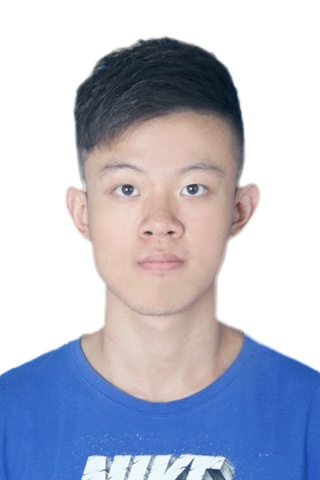
\includegraphics[width=1in,height=1.25in,clip,keepaspectratio]{bio/chenhao.jpg}}]{Hao Chen}
	received the B.S. degree in Internet of Things Engineering, in 2021, from the School of Physics and Information Engineering of Fuzhou University, Fuzhou, China. He is currently working towards the M.S. degree in Information Engineering at the School of Informatics, Xiamen University, Xiamen, China. His research interests include wireless communications.
\end{IEEEbiography}
\begin{IEEEbiography}[{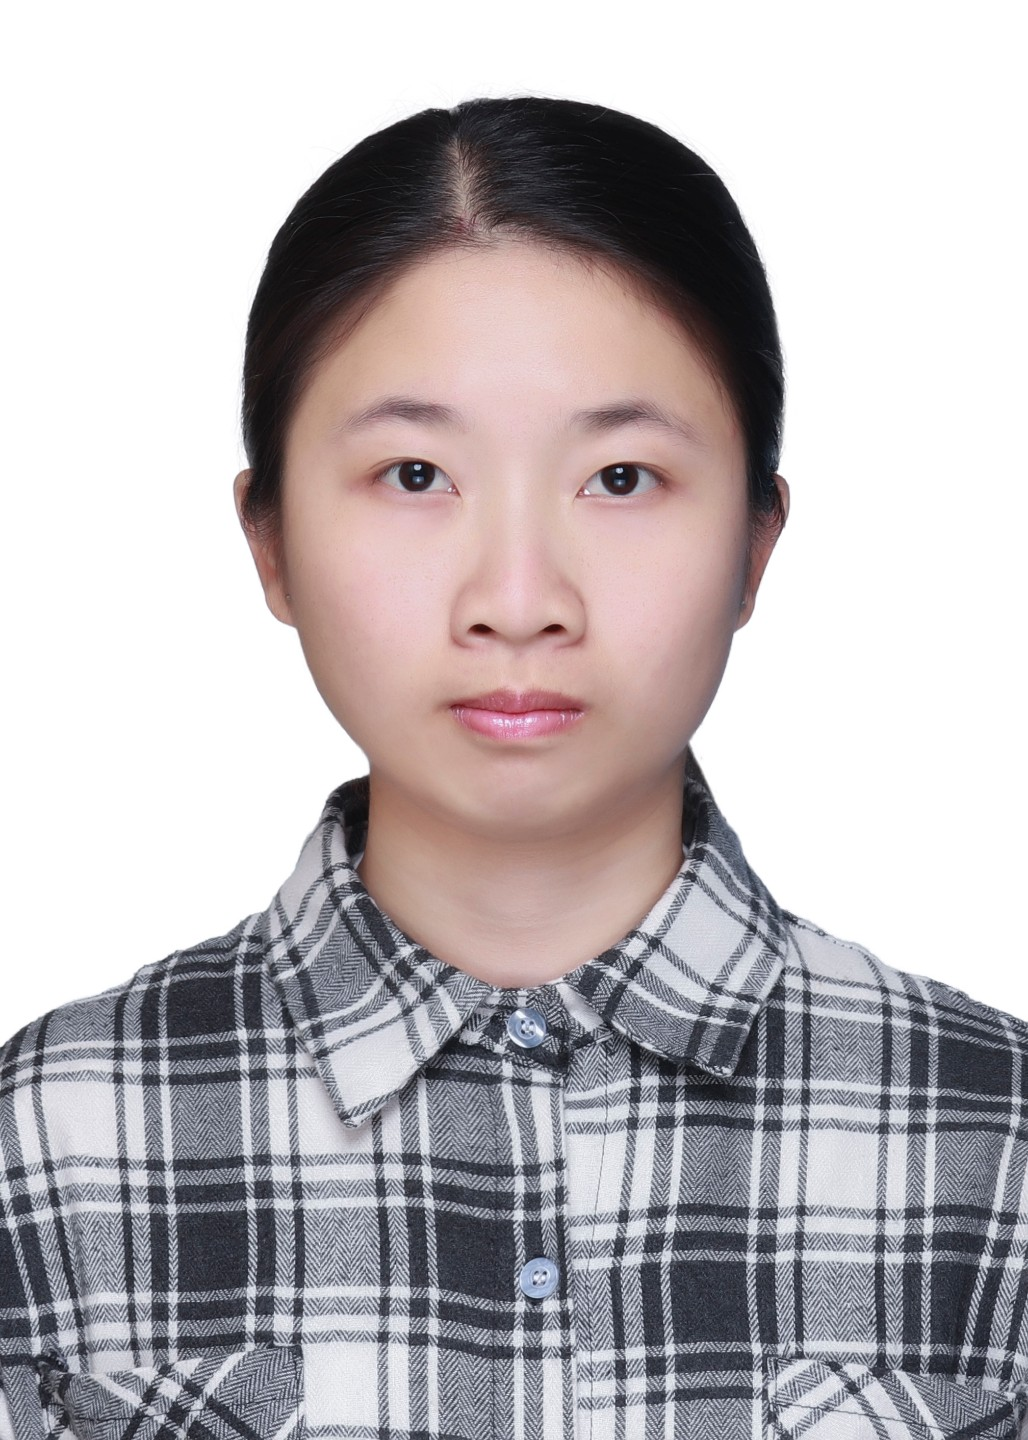
\includegraphics[width=1in,height=1.25in,clip,keepaspectratio]{bio/xiaoying.jpg}}]{Xiaoying Ye}
	received the B.S. degree in Communication Engineering, in 2021, from the School of Physics and Information Engineering of Fuzhou University, Fuzhou, China. She is currently working towards the M.S. degree in Information Engineering at the School of Informatics, Xiamen University, Xiamen, China. 
\end{IEEEbiography}

\begin{IEEEbiography}[{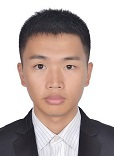
\includegraphics[width=1in,height=1.25in,clip,keepaspectratio]{bio/lizhao.jpg}}]{Lizhao You}
	received his B.S. and M.E. degrees from Nanjing University, China, in 2009 and 2013, and the Ph.D. degree from The Chinese University of Hong Kong, China, in 2016. He joined Huawei Technologies Co., Ltd. after his graduation until 2021. He is currently an Assistant Professor at Xiamen University, China. His research interests include wireless communications, computer networks and network verification.
\end{IEEEbiography}

\begin{IEEEbiography}[{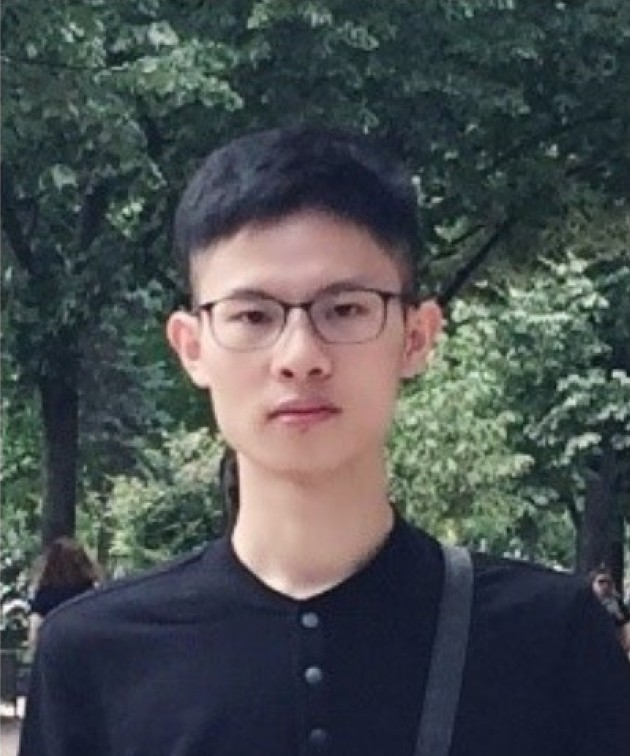
\includegraphics[width=1in,height=1.25in,clip,keepaspectratio]{bio/yulin.jpg}}]{Yulin Shao}
	received his B.S. and M.S. degrees from Xidian University (Hons.) in 2013 and 2016, and the Ph.D. degree from The Chinese University of Hong Kong (CUHK) in 2020. He was a research assistant with the Institute of Network Coding, a visiting scholar at Massachusetts Institute of Technology, and a postdoctoral fellow at CUHK. He is currently a research associate at Imperial College London. His research interests include wireless communications and machine learning.
\end{IEEEbiography}




\end{document}
